\chapter{Bilder, Tabellen und Formeln}
\section{Bilder}
Wie man Bilder einfügen kann, wird hier genauestens beschrieben:\\ \url{https://www.overleaf.com/learn/latex/Inserting_Images}

Um die Übersicht in der Dateistruktur zu wahren, ist es sinnvoll alle Bilder in einen eigenen Ordner zu packen.    
    
Bilder werden über den Befehl \verb+\includegraphics[0.75\textwidth]{Bilder/bild}+ eingefügt. Dabei kann die Dateiendung weggelassen werden.  Über die Parameter lässt sich bspw. die Größe des Bilds festlegen. 
Als Dateiformate eignen sich insbesondere pdf und eps (jpg und png sind auch möglich). Für svg-Grafiken wird \verb+\includesvg[PARAMETER]{SVG_NAME}+ genutzt.

Wird \verb+\includegraphics+ innerhalb einer \texttt{figure}-Umgebung aufgerufen, kann die Grafik mit \verb+\caption{TEXT}+ mit einer Bildunterschrift und mit \verb+\label{TEXT}+ mit einem Label versehen werden. Anschließend kann später auf das Bild mit \verb+\ref{TEXT}+ verwiesen werden. 


\begin{figure}[h]
\centering
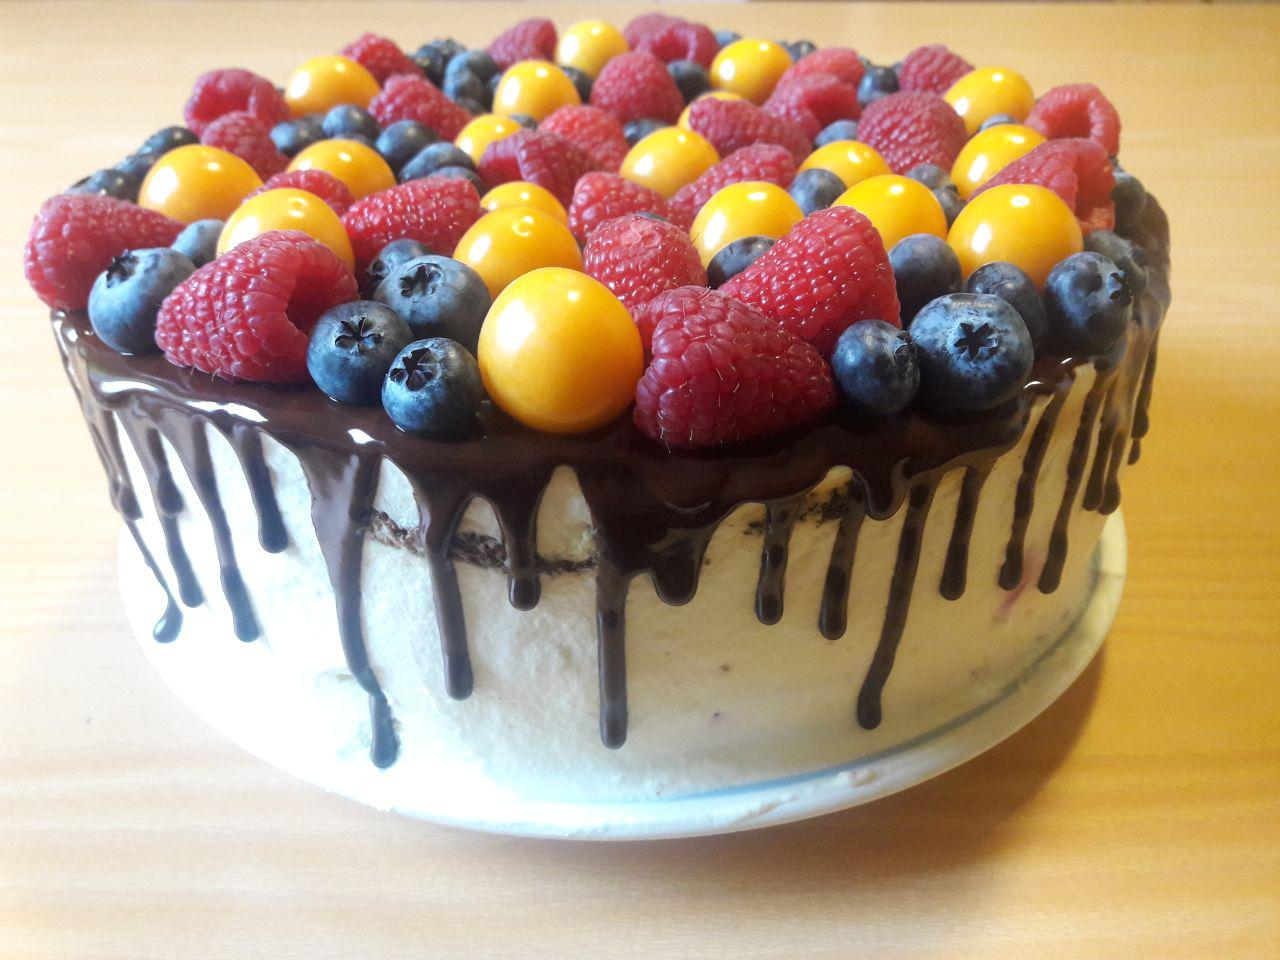
\includegraphics[width = 0.65\textwidth]{Bilder/torte1}
\caption{Leckere Torte}
\end{figure}

Um nur einen Bildausschnitt einzufügen, können die Parameter trim und clip zusammen verwendet werden. \verb+trim = left bottom right top+ gibt an, um wie viele cm jede Seite getrimmt werden soll.
Insgesamt ergibt sich dann für die Parameter bspw. \verb+[trim = 6cm 1cm 6cm 1cm, clip, width = 0.40\textwidth]+


\begin{figure}[h]
\centering
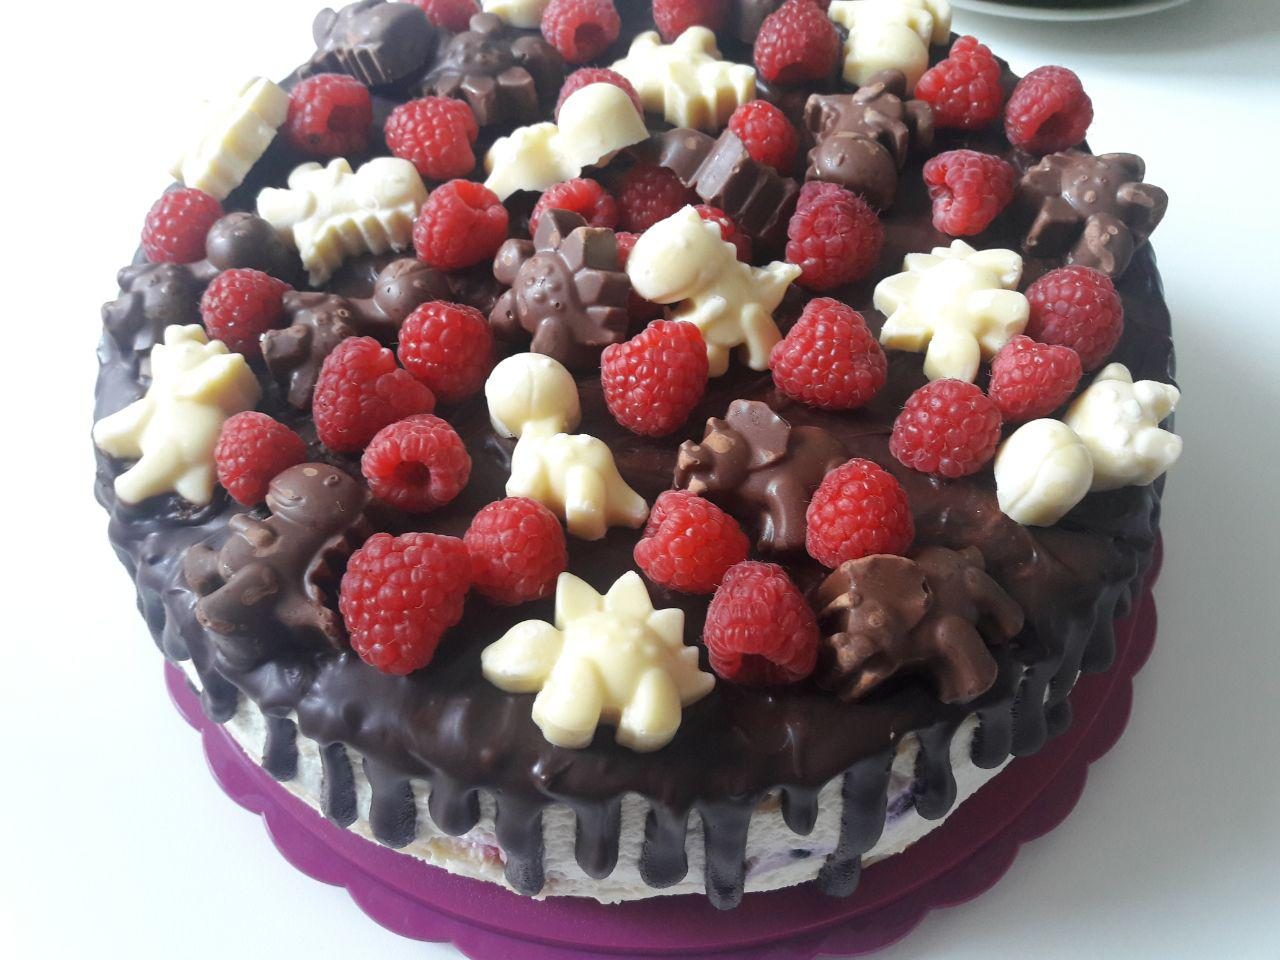
\includegraphics[trim = 6cm 3cm 6cm 1cm,clip , width = 0.35\textwidth]{Bilder/dinotorte}
\caption{Dino-Torte}
\end{figure}

Sollen (mehrere) ganze Seiten eines externen PDF-Dokuments eingefügt werden, kann der Befehl \verb+\includepdf[pages = {2,4,6-8}]{PDF_NAME}+ genutzt werden. 

\smallskip
Um zwei (oder mehr) Bilder nebeneinander auszugeben, können subfigures genutzt werden. Beispielcode dazu befindet sich in Anhang \ref{code_subfig}
\begin{figure}[h]
     \centering
     \begin{subfigure}[b]{0.55\textwidth}
         \centering
         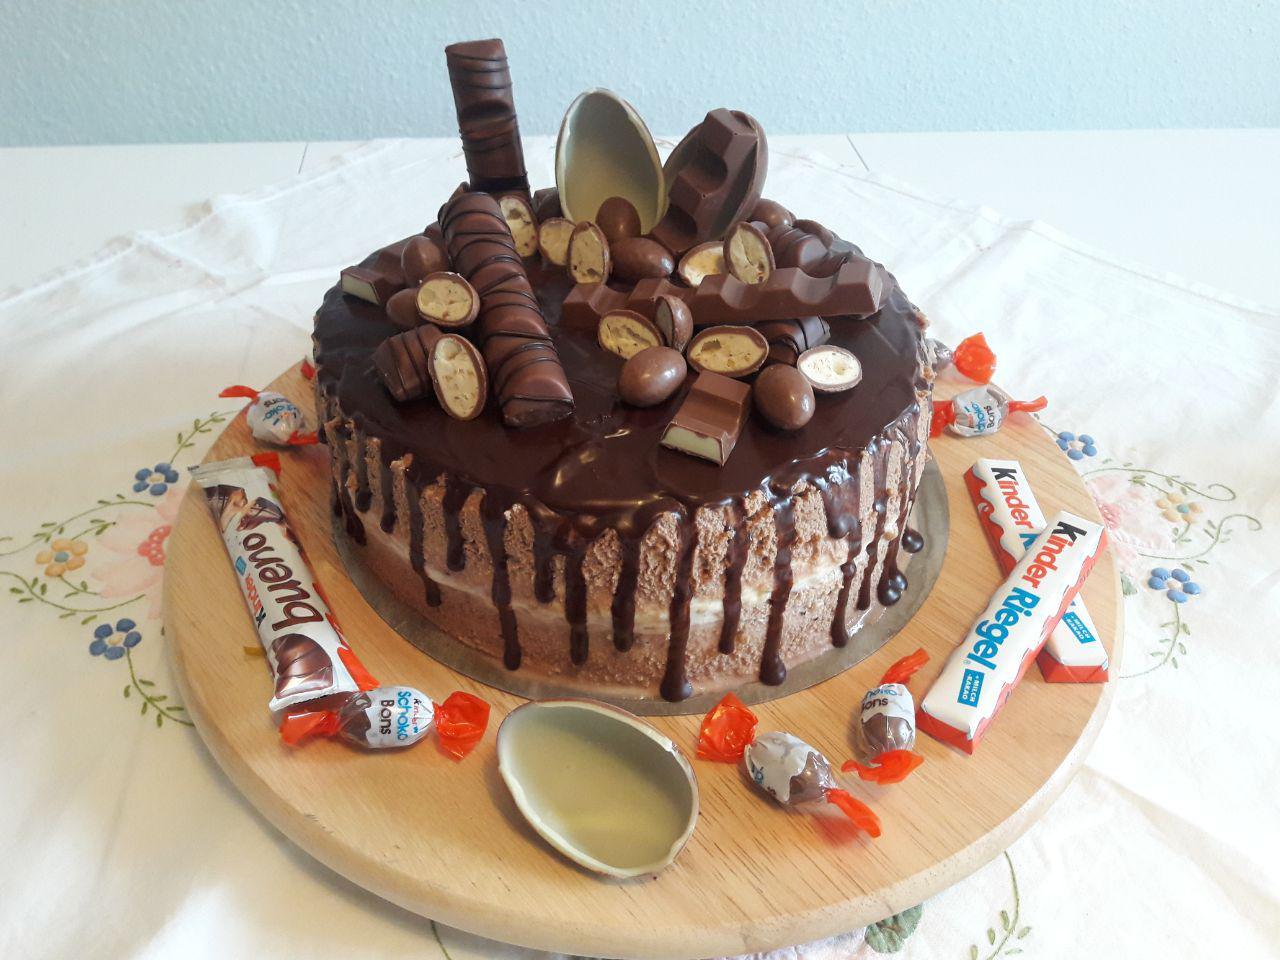
\includegraphics[width=\textwidth]{Bilder/kindertorte}
         \caption{Kinder-Torte}
         \label{fig:2_Bilder_Bild_1}
     \end{subfigure}
     \hfill
     \begin{subfigure}[b]{0.31\textwidth}
         \centering
         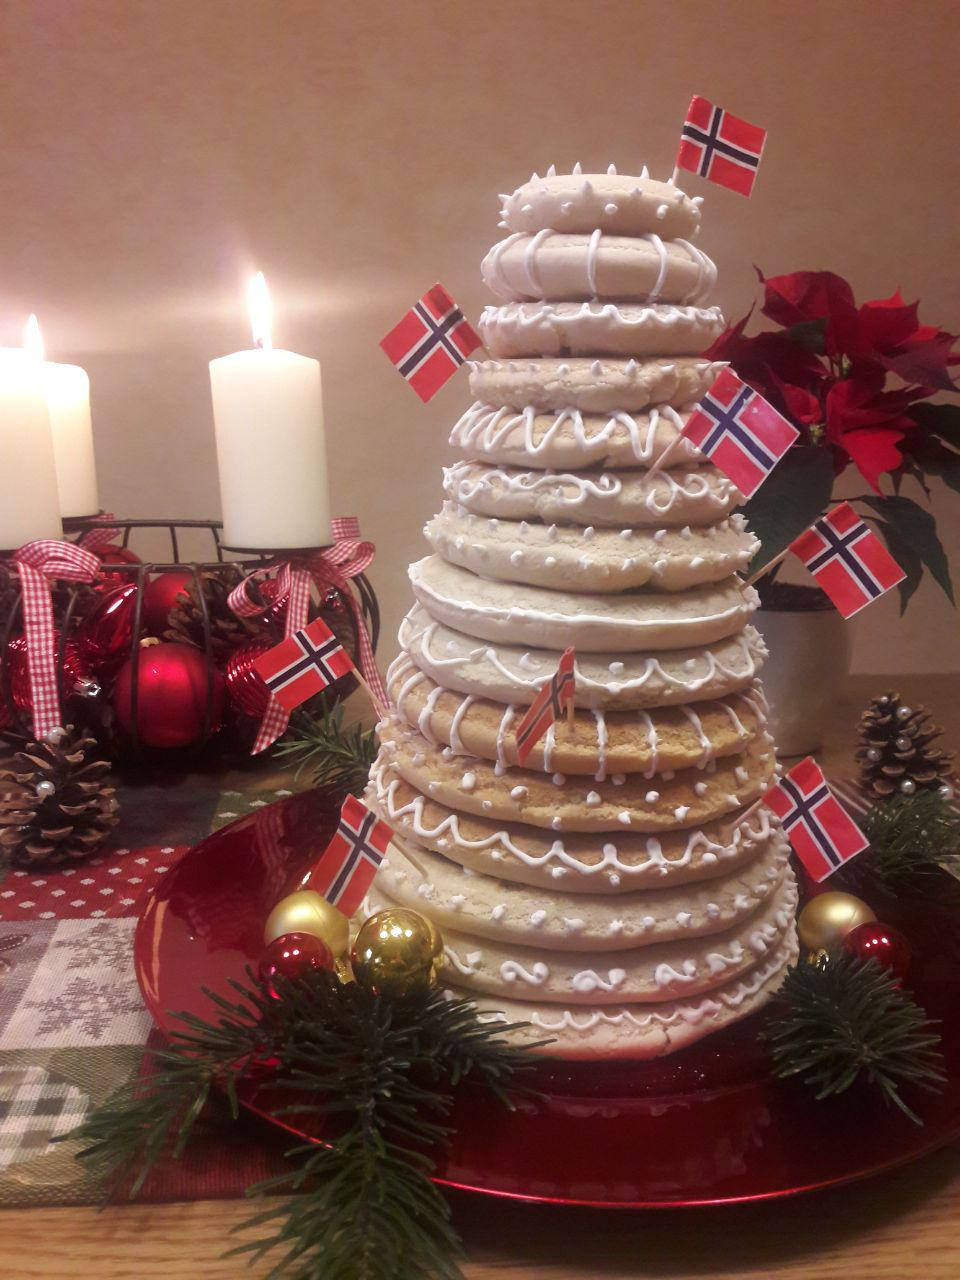
\includegraphics[width=\textwidth]{Bilder/kransekake}
         \caption{Kransekake}
         \label{fig:2_Bilder_Bild_2}
     \end{subfigure}
     \caption{Was schmeckt besser?}
\end{figure}

Für textumflossene Bilder kann die \texttt{floatingfigure}-Umgebung anstelle der \texttt{figure}-Umgebung genutzt werden. 
\verb+\begin{floatingfigure}[r\l\p]{width}+.


Dabei lässt sich die Platzierung des Bilds über die Parameter einstellen, r für rechts, l für links und p für Platzierung abhängig von der Seitenzahl.
\begin{floatingfigure}[l]{0.4\textwidth}
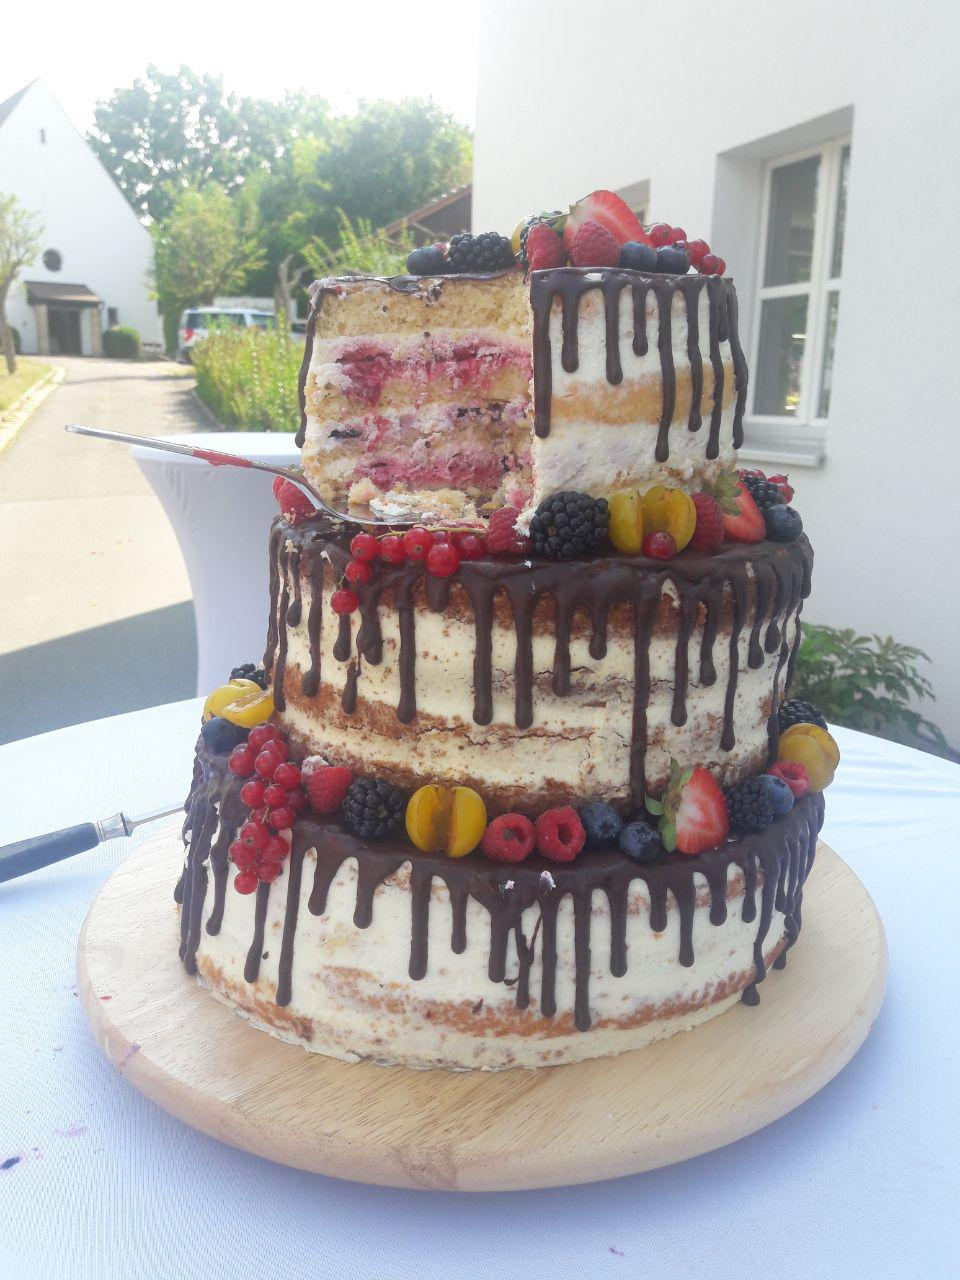
\includegraphics[width = 0.35\textwidth]{Bilder/hochzeitstorte}
\caption{Hochzeitstorte}
\end{floatingfigure} 
Mit width wird die Breite des Platzes, welcher für das Bild vorgesehen ist, festgelegt. 
Im Inneren der Umgebung wird das Bild wie gewohnt eingefügt. Auch eine Caption kann hier verwendet werden.
Die dort eingestellte Breite sollte zu der der floatingfigure passen. 
Schreibt man jetzt weiterhin Text, wird dieser neben dem Bild ausgegeben. Dabei sollte eine floatingfigure nicht zu nah an bspw. einer neuen Section platziert werden. Hier kommt es zur Kollision. Daher steht hier jetzt noch etwas unnötiger Text um den Abstand zum nächsten Kapitel zu vergrößern. Unnötiger Text und Kuchenbilder haben in Abschlussarbeiten aber in den meisten Fällen nichts zu suchen. Jetzt braucht es noch einen Satz, um das Bild vollständig zu überbrücken und zu zeigen, dass es danach wieder mit dem normalen Einzug weiter geht. 

Zur Einbindung von Formeln in Abbildungen empfiehlt sich Ti\textit{k}Z. Ein Editor zur Erstellung solcher Abbildung ist \emph{The Ipe extensible drawing editor} (\url{http://ipe.otfried.org/}). Durch Einbindung der \emph{ipe2tikz}-Erweiterung (\url{https://github.com/QBobWatson/ipe2tikz}) können so Vektorgrafiken erzeugt werden, die Formeln enthalten.
\begin{figure}[h]
	\centering
	\begin{tikzpicture}[scale=1.0, every node/.style={scale=1.0}]
	\tikzstyle{ipe stylesheet} = [
  ipe import,
  even odd rule,
  line join=round,
  line cap=butt,
  ipe pen normal/.style={line width=0.4},
  ipe pen heavier/.style={line width=0.8},
  ipe pen fat/.style={line width=1.2},
  ipe pen ultrafat/.style={line width=2},
  ipe pen normal,
  ipe mark normal/.style={ipe mark scale=3},
  ipe mark large/.style={ipe mark scale=5},
  ipe mark small/.style={ipe mark scale=2},
  ipe mark tiny/.style={ipe mark scale=1.1},
  ipe mark normal,
  /pgf/arrow keys/.cd,
  ipe arrow normal/.style={scale=7},
  ipe arrow large/.style={scale=10},
  ipe arrow small/.style={scale=5},
  ipe arrow tiny/.style={scale=3},
  ipe arrow normal,
  /tikz/.cd,
  ipe arrows, % update arrows
  <->/.tip = ipe normal,
  ipe dash normal/.style={dash pattern=},
  ipe dash dashed/.style={dash pattern=on 4bp off 4bp},
  ipe dash dotted/.style={dash pattern=on 1bp off 3bp},
  ipe dash dash dotted/.style={dash pattern=on 4bp off 2bp on 1bp off 2bp},
  ipe dash dash dot dotted/.style={dash pattern=on 4bp off 2bp on 1bp off 2bp on 1bp off 2bp},
  ipe dash normal,
  ipe node/.append style={font=\normalsize},
  ipe stretch normal/.style={ipe node stretch=1},
  ipe stretch normal,
  ipe opacity 10/.style={opacity=0.1},
  ipe opacity 30/.style={opacity=0.3},
  ipe opacity 50/.style={opacity=0.5},
  ipe opacity 75/.style={opacity=0.75},
  ipe opacity opaque/.style={opacity=1},
  ipe opacity opaque,
]
\begin{scope}[ipe stylesheet]
  \draw[shift={(232, 608)}, xscale=0.75]
    (0, 0) rectangle (64, -32);
  \draw
    (196, 592) circle[radius=4];
  \node[ipe node, anchor=north west]
     at (239, 596) {
       \begin{minipage}{60bp}\kern0pt
         Regler
       \end{minipage}
     };
  \draw[-{>[ipe arrow small]}]
    (164, 592)
     -- (192, 592);
  \draw[shift={(320.1, 608)}, xscale=0.7496]
    (0, 0) rectangle (64, -32);
  \node[ipe node, anchor=north west]
     at (328.1, 596) {
       \begin{minipage}{52bp}\kern0pt
         Strecke
       \end{minipage}
     };
  \node[ipe node]
     at (392, 599) {$y(t)$};
  \draw[shift={(400, 592)}, xscale=1.275, -{>[ipe arrow small]}]
    (0, 0)
     -- (0, -32)
     -- (-160, -32)
     -- (-160, -4);
  \filldraw[black]
    (400, 592) circle[radius=1];
  \draw[shift={(200.001, 592)}, xscale=2.6667, -{>[ipe arrow small]}]
    (0, 0)
     -- (12, 0);
  \draw[shift={(400.001, 592)}, xscale=2.6667, -{>[ipe arrow small]}]
    (0, 0)
     -- (12, 0);
  \draw[shift={(368.001, 592)}, xscale=2.6667]
    (0, 0)
     -- (12, 0);
  \draw[shift={(280.003, 592)}, xscale=3.3334, -{>[ipe arrow small]}]
    (0, 0)
     -- (12, 0);
  \node[ipe node]
     at (292, 599) {$u(t)$};
  \node[ipe node]
     at (208, 599) {$e(t)$};
  \node[ipe node]
     at (164, 599) {$w(t)$};
  \draw
    (200, 584)
     -- (204, 584);
  \draw[-{>[ipe arrow small]}]
    (344, 624)
     -- (344, 608);
  \node[ipe node]
     at (336, 631) {$z(t)$};
\end{scope}

	\end{tikzpicture}
	\caption{Standardregelkreis, erstellt mit dem Ti\textit{k}Z-Editor \emph{Ipe}} \label{fig:Standardregelkreis}
\end{figure}

\section{Tabellen}
Eine Anleitung zu Tabellen findet man hier: \url{https://www.overleaf.com/learn/latex/Tables}. 

Eine einfache Tabelle lässt sich mit Hilfe der \texttt{tabular}-Umgebung erzeugen: 

\begin{center}
\begin{verbatim}
\begin{table}[h]
\centering
\begin{tabular}{ c c c c }
\hline
 h1  & h2  & h3  & h4	\\ \hline
 t1  & t2  & t3  & t4	\\
 t5  & t6  & t7  & t8	\\  
 t9  & t10 & t11 & t12 \\ 
 t13 & t14 & t15 & t16 \\ \hline
\end{tabular}
\caption{einfache Tabelle}
\label{tab:tab1}
\end{table}
\end{verbatim}
\end{center}

\begin{table}[h]
\centering
\begin{tabular}{ c c c c }
\hline
 h1  & h2  & h3  & h4   \\ \hline
 t1  & t2  & t3  & t4   \\
 t5  & t6  & t7  & t8   \\  
 t9  & t10 & t11 & t12 	\\ 
 t13 & t14 & t15 & t16 	\\ \hline
\end{tabular}
\caption{einfache Tabelle}
\label{tab:tab1}
\end{table}

Die Parameter der tabular-Umgebung geben an, wie viele Spalten die Tabelle hat und wie diese jeweils ausgerichtet sind (l,c,r).  Durch Einfügen eines $\vert$ zwischen den Parametern lassen sich senkrechte Striche zwischen den Spalten einfügen. Für horizontale Trennstriche wird der Befehl \verb+\hline+ genutzt. Außerdem kann\verb+ \cline{x-y}+ genutzt werden, um den Strich nur von Spalte x bis y einzuzeichnen.


Um mehrere Reihen oder Spalten zusammenzufassen, können \verb+\multirow{•}{•}{•}+ und \verb+\multicolumn{•}{•}{•}+ verwendet werden. Dabei gibt der erste Parameter die Anzahl der Spalten/Reihen an die überspannt werden sollen, der zweite die Formatierung der Zelle, bzw. im Fall von Reihen die Breite der Spalte und der letzte den Inhalt der Zelle an. 

\begin{table}[h]
\centering
\begin{tabular}{ |c| c| c |}
\hline
\multicolumn{3}{|c|}{Kopf}\\
\hline
 & t2 & t3 \\ 
 \cline{2-3}
  \multirow{-2}*{t14} & t5 &\multicolumn{1}{c}{} \\  
 \cline{1-2}
 t7 &  t8 & \multicolumn{1}{c}{\multirow{-2}*{t69}}\\
\cline{1-2}
\end{tabular}
\caption{etwas ausgefallenere Tabelle}
\end{table}

Wie bei Bildern, lassen sich auch Tabellen durch \texttt{subtable} in der \texttt{table}-Umgebung nebeneinander darstellen. 
\newpage
\section{Formeln und Gleichungen}
Ein kleiner Einstieg ist hier: \url{https://www.overleaf.com/learn/latex/Mathematical_expressions} zu finden.
Für Gleichungen und Formeln gibt es eine Vielzahl verschiedener Möglichkeiten zur Umsetzung.

Einfache mathematische Ausdrücke, die in den Fließtext eingebunden werden sollen, können wie \(a=b\) in der Form \verb+\(a=b\)+ oder in einfachen Dollarzeichen \verb+$a=b$+ eingefügt werden.

Um die Formel in einer eigenen Zeile auszugeben, werden entweder doppelte Dollarzeichen \verb+$$a=b$$+ oder \verb+\[a=b\]+ verwendet.$$a=b$$ Alternativ kann auch die \texttt{equation}-Umgebung genutzt werden. 
\begin{equation}
a=b
\end{equation}
Wie bei der \texttt{figure}-Umgebung lässt sich auch hier ein Label vergeben. Unabhängig davon wird die Gleichungsnummer neben der Gleichung ausgegeben. Soll die \texttt{equation}-Umgebung ohne Nummerierung verwendet werden, kann diese mit \verb+\nonumber+ am Ende der Gleichung unterdrückt werden.  

\smallskip
Sollen mehrere Gleichungen untereinander ausgerichtet werden, kann die \texttt{align}-Umgebung genutzt werden. Dabei können mit \verb+&+ die Stellen markiert werden, an denen ausgerichtet werden soll. 
\begin{align}
a&=b-c\\
b-d&=d\cdot e\\
&=f
\end{align}

\begin{verbatim}
\begin{align}
a&=b-c\\
b-d&=d\cdot e\\
&=f
\end{align}
\end{verbatim}

Um nur eine Gleichungsnummer für alle Gleichungen zusammen auszugeben, wird der Befehl \verb+split+ verwendet.

\begin{align}
\begin{split}
a&=b-c\\
b-d&=d\cdot e\\
&=f
\end{split}
\end{align}

\begin{verbatim}
\begin{align}
\begin{split}
a&=b-c\\
b-d&=d\cdot e\\
&=f
\end{split}
\end{align}
\end{verbatim}


Für Matrizen werden je nach gewünschter Klammer \verb+pmatrix+ oder \verb+bmatrix+ verwendet. Als pmatrix besitzt die Matrix runde Klammern, als bmatrix eckige. 
\begin{align}\text{pmatrix:} &&
\begin{pmatrix}
a_{1,1} & \dots & a_{1,n}\\
\vdots & \ddots & \vdots \\
a_{m,1} & \dots & a_{m,n}
\end{pmatrix} \nonumber
\end{align}


\begin{align}\text{bmatrix:} &&
\begin{bmatrix}
a_{1,1} & \dots & a_{1,n}\\
\vdots & \ddots & \vdots \\
a_{m,1} & \dots & a_{m,n}
\end{bmatrix} \nonumber
\end{align}


Im Inneren sind die Matrizen wie Tabellen aufgebaut. Die Punkte lassen sich mit \verb+\dots+, \verb+\vdots+ und \verb+\ddots+ erzeugen.  

